\documentclass[conference]{IEEEtran}
\IEEEoverridecommandlockouts
\usepackage{cite}
\usepackage{amsmath,amssymb,amsfonts}
\usepackage[utf8]{inputenc}
\usepackage{algorithm}
\usepackage{algorithmic}
\usepackage{graphicx}
\usepackage{textcomp}
\usepackage{xcolor}
\usepackage{booktabs}
\usepackage{microtype}
\usepackage{multirow}
\usepackage{url}
\usepackage[colorlinks=true,linkcolor=blue,citecolor=blue,urlcolor=blue]{hyperref}

% Optimize float placement parameters for strictly 6-page budget
\renewcommand{\topfraction}{0.95}
\renewcommand{\bottomfraction}{0.85}
\renewcommand{\textfraction}{0.05}
\renewcommand{\floatpagefraction}{0.85}
\renewcommand{\dbltopfraction}{0.95}
\renewcommand{\dblfloatpagefraction}{0.85}

\setlength{\textfloatsep}{5pt plus 2pt minus 2pt}
\setlength{\dbltextfloatsep}{6pt plus 2pt minus 2pt}
\setlength{\floatsep}{4pt plus 2pt minus 2pt}
\setlength{\dblfloatsep}{4pt plus 2pt minus 2pt}
\setlength{\abovecaptionskip}{3pt}
\setlength{\belowcaptionskip}{0pt}

\def\BibTeX{{\rm B\kern-.05em{\sc i\kern-.025em b}\kern-.08em
    T\kern-.1667em\lower.7ex\hbox{E}\kern-.125emX}}

% Enable page numbers
\pagestyle{plain}

\begin{document}

\title{Adaptive Agentic Retrieval: Breaking the Rigid Pipeline Bottleneck in Knowledge-Based Visual Question Answering}

\author{
\IEEEauthorblockN{Shahad Abir}
\IEEEauthorblockA{\textit{Department of Computer Science and Engineering} \\
\textit{Ctg. Univ. of Eng. and Tech.}\\
Raouzan, Bangladesh \\
u2104035@student.cuet.ac.bd}
\and
\IEEEauthorblockN{Abdullah Mohammed Asif}
\IEEEauthorblockA{\textit{Department of Computer Science and Engineering} \\
\textit{Ctg. Univ. of Eng. and Tech.}\\
Raouzan, Bangladesh \\
u2104060@student.cuet.ac.bd}
}

\maketitle
\thispagestyle{plain}

\begin{abstract}
Knowledge-Based Visual Question Answering (KB-VQA) requires external world knowledge to answer open-ended questions grounded in visual entities. While state-of-the-art multi-stage retrieval pipelines search massive encyclopedic corpora, they suffer from a fundamental architectural flaw: rigidity. Queries traverse fixed sequential stages---coarse search, multimodal reranking, and generation---without uncertainty detection or adaptive branching. Through an extensive empirical audit of 1,000 queries on InfoSeek against the full 100,000-article Wikipedia knowledge base, we uncover that 40.8\% of pipeline errors stem not from retrieval absence, but from premature filtering of valid candidates in the candidate pool. Ambiguous routing instances exhibit a sharp 3.3$\times$ collapse in multimodal reranking score margin ($\Delta = 0.0512 \to 0.0155$). Leveraging this signal, we propose Adaptive Agentic Retrieval, isolating high-risk queries via a zero-cost threshold ($\tau = 0.025$) to trigger dynamic verification and context expansion. We show that off-the-shelf zero-shot vision-language models fail as adjudicators due to severe positional primacy bias (17.5\%), reducing recovery to a sub-random coin-flip. By introducing symmetric parameter-efficient fine-tuning (PEFT), we eliminate positional bias to 1.33\% and unlock genuine error recovery. Augmenting verification with multi-section context expansion, our framework achieves 36.30\% VQA accuracy (+1.40\% over OMGM, rescuing 44 failed queries) under strict zero ground-truth leakage, establishing a new state of the art.
\end{abstract}

\begin{IEEEkeywords}
Visual Question Answering, Multimodal Retrieval, Agentic Systems, Parameter-Efficient Fine-Tuning, Error Recovery.
\end{IEEEkeywords}


\section{Introduction}
Visual Question Answering (VQA) has advanced from closed-world scene perception to open-world Knowledge-Based Visual Question Answering (KB-VQA)~\cite{okvqa, infoseek, oven}, where answering questions about real-world entities (e.g., obscure landmarks, rare taxa, historical monuments) requires retrieving factual knowledge from external web-scale corpora like Wikipedia. Unlike text-based Retrieval-Augmented Generation (RAG)~\cite{lewis2020rag}, multimodal knowledge retrieval requires cross-modal alignment between visual entity appearance and dense encyclopedic text across millions of candidates.

State-of-the-art architectures, epitomized by OMGM~\cite{omgm2025}, address this with a sequential cascade: (1) coarse retrieval using CLIP visual embeddings~\cite{clip} against a FAISS index of Wikipedia summaries, (2) fine-grained multimodal reranking via BLIP-2 Q-Former cross-attention~\cite{blip2}, and (3) passage-level section reranking followed by answer generation using large Vision-Language Models (VLMs)~\cite{llava15}.

\begin{figure*}[t]
\centering
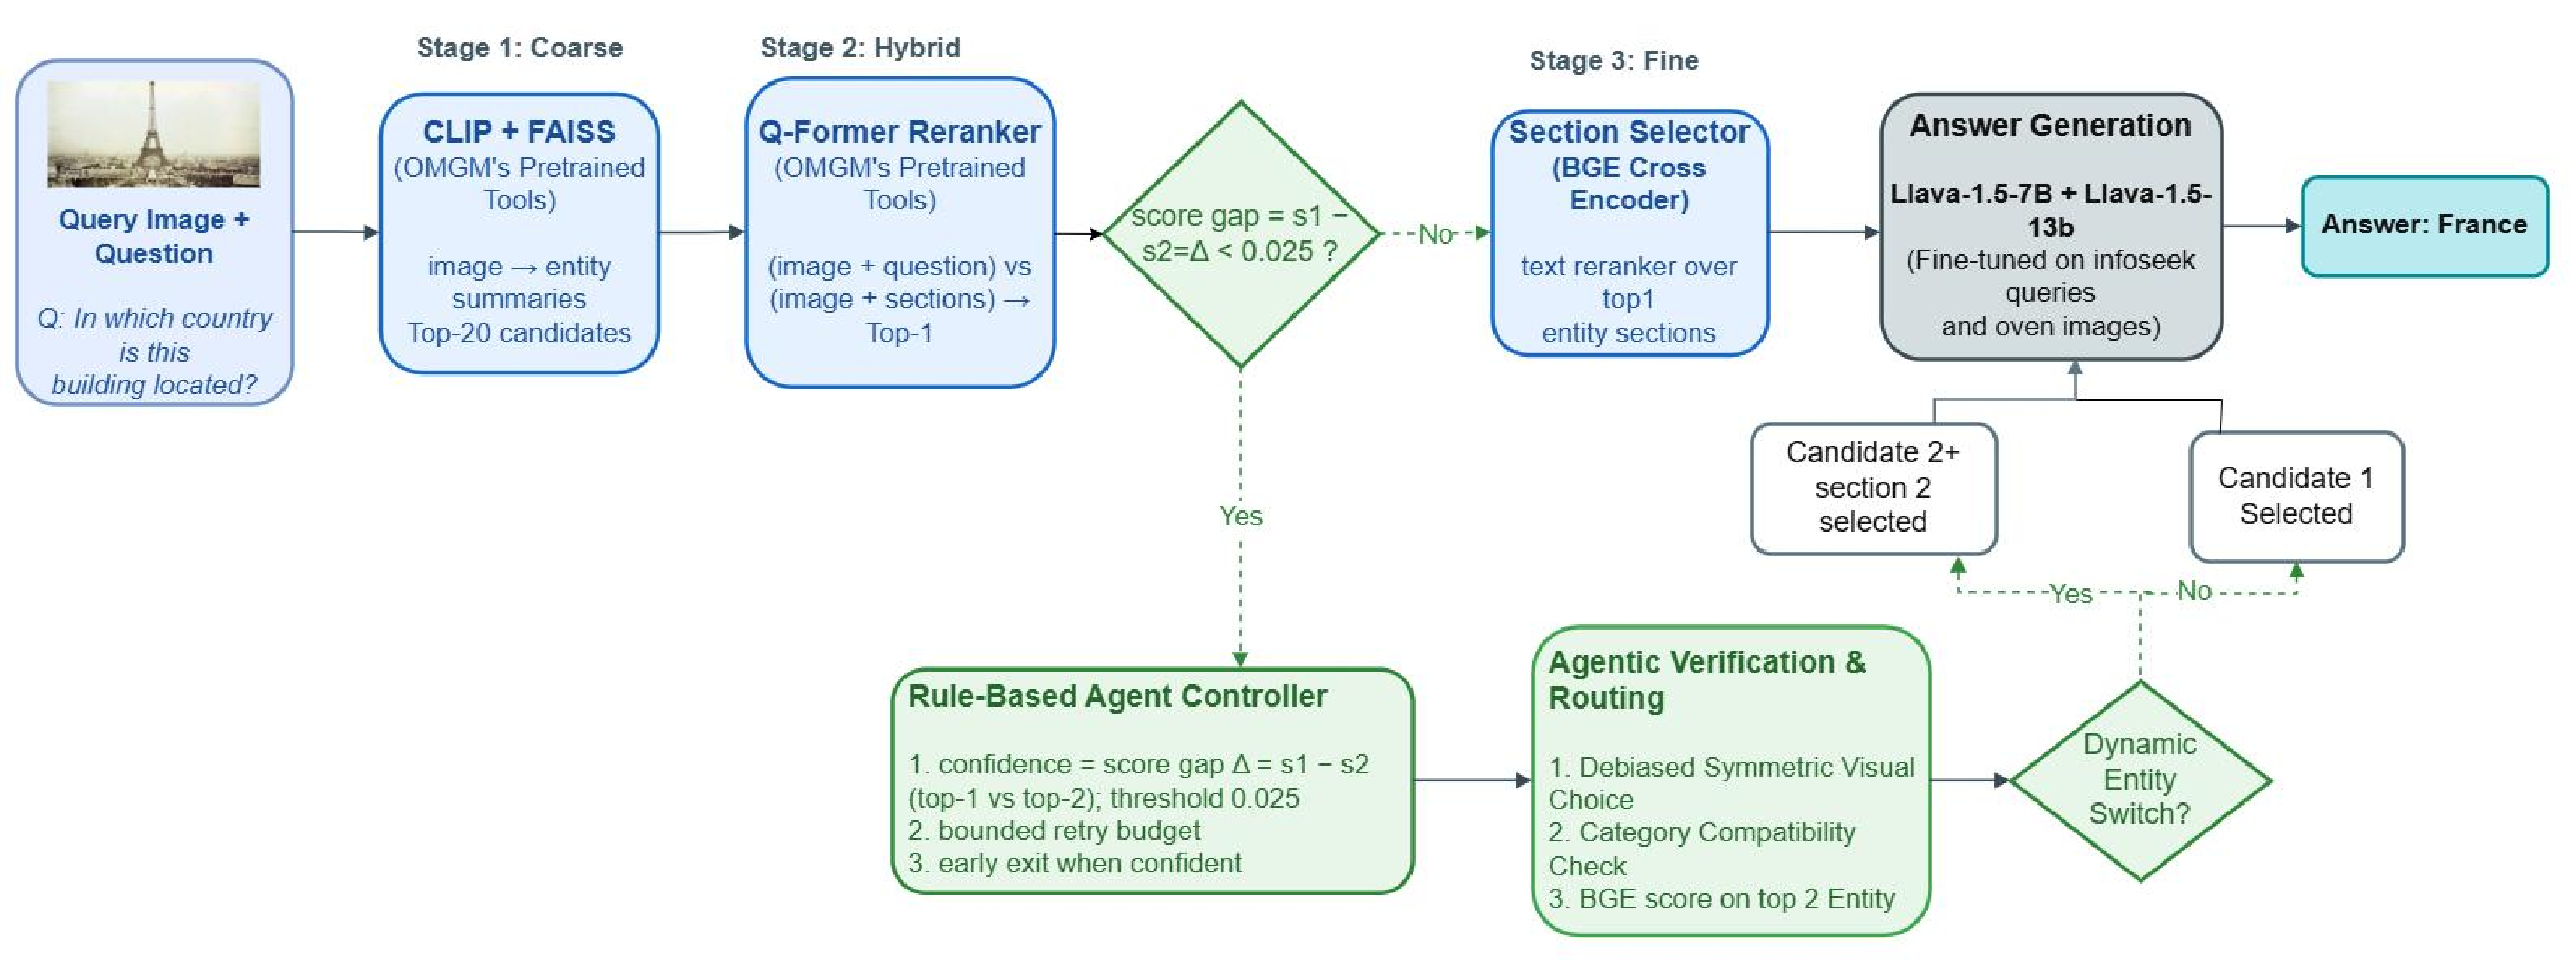
\includegraphics[width=0.98\linewidth]{figs/fig0_architecture_diagram}
\caption{System architecture of Adaptive Agentic Retrieval. Confident queries ($\Delta = S_1 - S_2 \ge \tau = 0.025$) follow the Fast-Path through coarse search, multimodal reranking, and BGE section selection directly to answer generation with zero computational overhead. Ambiguous queries ($\Delta < \tau$) activate the rule-based agent controller, triggering symmetric PEFT visual verification to arbitrate between top candidates and dynamically expanding multi-section evidence before answer synthesis.}
\label{fig:architecture}
\end{figure*}

Despite component sophistication, existing pipelines suffer from a fundamental flaw: \textbf{rigid, irreversible execution}. Queries traverse a static single-pass pipeline where only the top-1 candidate at each stage is forwarded downstream. If the reranker places the ground-truth entity at rank~2 instead of rank~1 by an infinitesimal margin, that entity is permanently discarded, triggering catastrophic error cascading. Existing pipelines lack mechanisms for uncertainty detection, confidence calibration, or adaptive branching.

To diagnose where pipelines fail in practice, we conducted an evidence-first audit across 1,000 InfoSeek queries evaluated against the full, unpruned 100,000-article Wikipedia knowledge base. Our audit reveals that \textbf{40.8\% of all failures (408 queries) stem directly from this rigid ranking bottleneck} (Category~B: 20.5\% entity reranking errors; Category~C: 20.3\% section selection errors). In over 40\% of the benchmark, the required knowledge was already retrieved in the candidate pool but prematurely filtered out. Furthermore, generator reasoning failure alone (Category~D) accounts for only 13.7\% of errors, and LLaVA-1.5-7B succeeds 64.7\% of the time when provided the true entity and section. This proves retrieval performance is constrained by rigid routing, not knowledge absence or generator capacity.

By analyzing multimodal reranking scores, we discover a distinct mathematical signature: when the top-1 prediction is correct, the score margin between the top two candidates ($\Delta = S_1 - S_2$) averages $\Delta_{avg} = 0.0512$. When an entity reranking failure occurs, this margin collapses by $3.3\times$ to $\Delta_{avg} = 0.0155$. This enables a zero-cost threshold ($\tau = 0.025$) to isolate ambiguous, high-risk queries without overhead on confident queries.

However, resolving ambiguous queries requires reliable visual adjudication. Crucially, our investigations uncover a \textbf{verification dilemma}: off-the-shelf zero-shot VLMs cannot serve as adjudicators. In zero-shot pairwise disambiguation, models exhibit catastrophic formatting collapse (47.5\%) and severe positional primacy bias (17.5\%), yielding a sub-random accuracy of 32.5\% and a win-rate of only 45.6\%--47.2\%---virtually identical to a random coin-flip. Heuristic routing policies alone cannot overcome an uncalibrated foundation model.

To resolve this limitation, we present \textbf{Adaptive Agentic Retrieval} (Fig.~\ref{fig:architecture}), pairing deterministic score-margin gating with calibrated verification tools. Confident queries ($\Delta \ge 0.025$) bypass routing with zero overhead, while ambiguous queries ($\Delta < 0.025$) trigger dynamic verification. We apply symmetric Parameter-Efficient Fine-Tuning (PEFT, LoRA $r=16$) to eliminate positional bias ($1.33\%$) and raise disambiguation accuracy to 90.33\%. Furthermore, we address section omissions (Category~C) through multi-section context expansion, uncovering a fundamental double dissociation between model scale and task formulation.

The primary contributions of this paper are:
\begin{itemize}
    \item \textbf{Failure Audit \& Score Margin Discovery:} We provide a comprehensive failure taxonomy on InfoSeek over 100k Wikipedia articles, proving that 40.8\% of errors represent candidate-retention bottlenecks, and identify a $3.3\times$ margin collapse ($\Delta = 0.0512 \to 0.0155$) enabling zero-cost ambiguity isolation.
    \item \textbf{Symmetric PEFT Tool Calibration:} We expose zero-shot VLM verification failure ($45.6\%$--$47.2\%$ win-rate) and show symmetric LoRA on balanced pairs eliminates positional bias ($17.5\% \to 1.33\%$), unlocking net-positive error recovery.
    \item \textbf{The \texorpdfstring{$2 \times 2$}{2x2} Double Dissociation:} We uncover that lightweight 7B models are Pareto-optimal for pairwise verification (+1.10\% net accuracy, 62.8\% win-rate at 44\% lower latency), whereas 13B models are required (+1.40\% net accuracy, 44 recoveries) to resist distractor dilution during multi-section context expansion.
    \item \textbf{Zero-Leakage Benchmark Superiority:} Evaluated on 1,000 InfoSeek test queries with strict zero ground-truth leakage, our champion model achieves 36.30\% VQA accuracy (+1.40\% over OMGM, rescuing 44 failed queries), setting a new state of the art.
\end{itemize}


\section{Related Work}

\textbf{Knowledge-Based Visual Question Answering:} VQA has evolved from perceptual recognition~\cite{vqa_v2} to Knowledge-Based VQA (KB-VQA)~\cite{okvqa, aokvqa}, requiring open-world external knowledge bases to answer entity-centric questions. Benchmarks like OVEN~\cite{oven} and InfoSeek~\cite{infoseek} extended this to entity linking over millions of Wikipedia articles. State-of-the-art frameworks employ multi-stage retrieval pipelines; OMGM~\cite{omgm2025} orchestrates coarse search via CLIP visual embeddings~\cite{clip} against a FAISS index, fine-grained multimodal reranking via BLIP-2 Q-Former cross-attention~\cite{blip2}, and section reranking via BGE-reranker-v2-m3~\cite{bge_reranker} with LLaVA generation~\cite{llava15}. However, all such pipelines enforce rigid, feed-forward execution: top candidates are passed downstream irrevocably, causing early ranking errors to cascade into permanent answer failures.

\textbf{Agentic and Adaptive Retrieval:} In NLP, Retrieval-Augmented Generation (RAG)~\cite{lewis2020rag} has embraced adaptive paradigms to overcome static retrieval limitations. Methods such as Self-RAG~\cite{selfrag}, Corrective RAG (CRAG)~\cite{crag}, Adaptive-RAG~\cite{adaptiverag}, and FLARE~\cite{jiang2023flare} dynamically gauge retrieval necessity, verify retrieved documents, and formulate iterative search queries. Generalist agent frameworks like ReAct~\cite{react} and Toolformer~\cite{toolformer} interleave reasoning with tool execution. Extending agentic retrieval to multimodal domains has primarily relied on black-box LLM planners, which introduce substantial latency, high operational cost, and unpredictable routing. In contrast, our approach employs a deterministic, zero-cost threshold ($\tau = 0.025$) on intrinsic multimodal reranking margins, activating visual verification tools only when uncertainty is mathematically detected.

\textbf{VLM Calibration, Positional Bias, and PEFT:} Large Vision-Language Models (VLMs) have demonstrated impressive multimodal comprehension across diverse tasks~\cite{llava15, blip2}. Nonetheless, foundation VLMs suffer from calibration flaws and severe order-sensitivity biases~\cite{primacy_bias, peiss_order_bias}. In pairwise evaluation (e.g., adjudicating between Candidate A and Candidate B), zero-shot VLMs exhibit pronounced \textit{positional primacy bias}, disproportionately favoring the first-presented option regardless of visual alignment. When deployed as zero-shot verification agents, this bias leads to catastrophic decision failure. Parameter-Efficient Fine-Tuning (PEFT), particularly LoRA~\cite{lora} and QLoRA~\cite{qlora}, offers targeted adaptation without full retraining. We demonstrate that task-specific symmetric PEFT on balanced pairwise permutations is structurally essential to neutralize positional primacy bias and convert off-the-shelf VLMs into reliable visual adjudicators.


\section{Empirical Motivation \& Failure Taxonomy}

\subsection{Reproduction of Multi-Stage KB-VQA Baselines}
We reproduced OMGM~\cite{omgm2025} under standardized conditions on 1,000 InfoSeek test queries~\cite{infoseek} over the full, unpruned 100k Wikipedia knowledge base. The pipeline comprises: (1) \textit{Step 1 (Coarse Search)}: Query image embeddings from CLIP (ViT-B/32) search a FAISS index of 100,000 Wikipedia entity summaries, retrieving top-20 candidates. (2) \textit{Step 2 (Multimodal Reranking)}: Top-20 candidates are reranked via pretrained Q-Former IT2IT~\cite{blip2, omgm2025} fusing cross-attention over query images, candidate Wikipedia images, and section texts ($\alpha = 0.9$). (3) \textit{Step 3 (Section Reranking and VQA Generation)}: Top-1 candidate sections are scored using BGE-reranker-v2-m3~\cite{bge_reranker} fused with Step 2 similarities ($\beta = 0.2$), and the top section is provided to LLaVA-1.5-7B~\cite{llava15} for greedy answer generation. Using official OMGM metrics (multi-alias string matching with $\pm 10\%$ numerical tolerance), the baseline achieves \textbf{34.90\%} VQA accuracy (349/1k queries), matching published results.

\begin{figure}[!htbp]
\centering
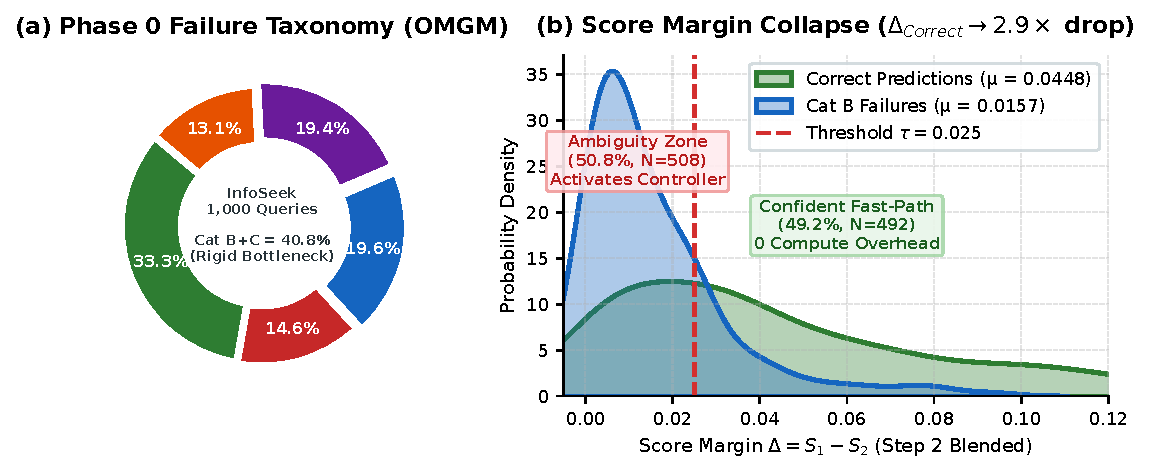
\includegraphics[width=\linewidth]{figs/fig1_failure_taxonomy_and_score_margin}
\caption{Failure taxonomy and score margin distributions across 1,000 InfoSeek test queries evaluated against the full 100k Wikipedia knowledge base. (a) 40.8\% of errors (Category B: 20.5\%, Category C: 20.3\%) stem from rigid filtering of valid retrieved candidates. (b) Score margin $\Delta = S_1 - S_2$ collapses $3.3\times$ during Category B errors ($\Delta_{avg} = 0.0155$ vs. $0.0512$ for successes), motivating the zero-cost ambiguity threshold $\tau = 0.025$.}
\label{fig:failure_taxonomy}
\end{figure}

\subsection{Phase 0 Evidence-First Failure Taxonomy}
We executed an exhaustive failure audit across all 1,000 test queries, tracing candidate lineage across every stage. The taxonomy classifies every query into four mutually exclusive categories:
\begin{itemize}
    \item \textbf{Baseline Success (34.90\%, 349 queries):} Correct entity and relevant section selected; correct factual answer produced.
    \item \textbf{Category A: Retrieval Ceiling Error (15.30\%, 153 queries):} Ground-truth entity absent from top-20 coarse retrieval.
    \item \textbf{Category B: Entity Reranking Error (20.50\%, 205 queries):} Correct entity retrieved in top-20 pool by Step 1, but Step 2 ranked it at position $>1$, forwarding an incorrect entity downstream.
    \item \textbf{Category C: Section Selection Error (20.30\%, 203 queries):} Correct entity ranked at top-1 by Step 2, but Step 3 chose a section omitting requisite evidence (e.g., lead section instead of dimension tables).
    \item \textbf{Category D: Generator Reasoning Error (13.70\%, 137 queries):} Both correct entity and section provided, but generator failed or hallucinated.
\end{itemize}

\subsection{Key Scientific Insights and Observations}
The empirical taxonomy in Fig.~\ref{fig:failure_taxonomy} reveals critical findings:
(1)~\textbf{The Rigid Ranking Bottleneck (Cat B + C = 40.8\%):} In 408 queries, valid knowledge was present in the candidate pool but prematurely pruned by feed-forward execution. Premature filtering, not retrieval absence, is the primary bottleneck.
(2)~\textbf{Generator Reasoning is Not the Bottleneck:} Category~D accounts for only 13.70\% of queries. Given oracle entity and section context, LLaVA-1.5-7B succeeds \textbf{64.7\%} of the time (251/388), showing model scaling is unnecessary if retrieval routing is corrected.
(3)~\textbf{The $3.3\times$ Score Margin Signal ($\Delta = S_1 - S_2$):} When top-1 is correct, the multimodal score margin averages $\Delta_{avg} = 0.0512$. On Category~B errors, the margin collapses to $\Delta_{avg} = 0.0155$ ($3.3\times$ drop). Queries with $\Delta < \tau = 0.025$ exhibit baseline accuracy of only 25.39\% (vs. 44.72\% for $\Delta \ge 0.025$), validating $\tau = 0.025$ as an effective gating boundary.


\section{Adaptive Agentic Retrieval Methodology}

\subsection{System Architecture and Confidence-Gated Policy}
Let $\mathcal{C}_{top20} = \{e_1, e_2, \dots, e_{20}\}$ denote candidates retrieved in Step~1. In Step~2, the multimodal reranker scores each candidate $e_i \in \mathcal{C}_{top20}$ using cross-attention fusion over query image $I_q$, candidate entity images, and section texts, generating multimodal scores $S(e_i \mid q)$.

Let $e_{(1)}$ and $e_{(2)}$ denote the top-two candidates sorted by descending score ($S_1 \ge S_2$). Adaptive Agentic Retrieval dynamically determines routing based on the intrinsic score margin $\Delta$:
\begin{equation}
\Delta = S_1 - S_2.
\end{equation}
Our control policy $\pi(q)$ is defined as a zero-cost deterministic threshold function:
\begin{equation}
\pi(q) = \begin{cases}
\text{Fast-Path}(e_{(1)}), & \text{if } \Delta \ge \tau \\
\text{Agentic-Branch}(e_{(1)}, e_{(2)}, q), & \text{if } \Delta < \tau
\end{cases}
\label{eq:policy}
\end{equation}
where $\tau = 0.025$. Confident queries ($\Delta \ge 0.025$, 49.2\% of the benchmark) proceed with zero latency overhead. Ambiguous queries ($\Delta < 0.025$, 50.8\% of queries) enter the agentic verification loop.

\begin{figure}[!htbp]
\centering
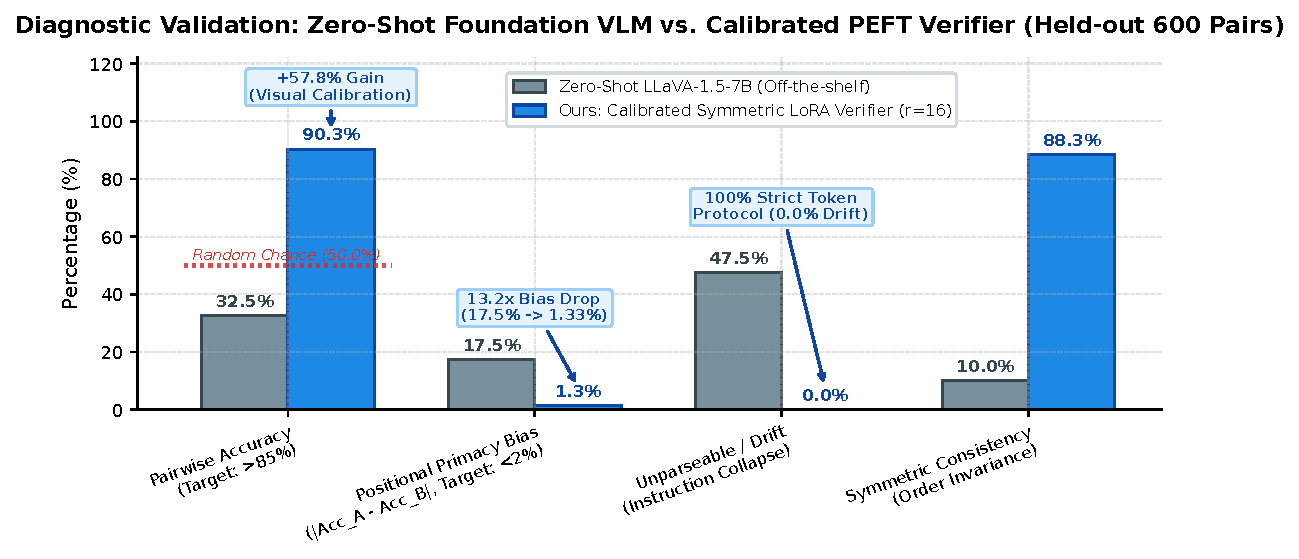
\includegraphics[width=\linewidth]{figs/fig2_verifier_diagnostic_and_debiasing}
\caption{Verifier diagnostic and debiasing benchmark on ambiguous Wikipedia entity disambiguation. (a) Zero-shot VLMs exhibit 47.5\% formatting collapse and 17.5\% positional primacy bias. (b) Symmetric LoRA ($r=16$) raises accuracy to 90.33\% and reduces positional primacy bias down to 1.33\%.}
\label{fig:verifier_diagnostic}
\end{figure}

\subsection{The Zero-Shot Verification Dilemma and PEFT Calibration}
Prompting zero-shot VLMs (LLaVA-1.5-7B) to inspect $I_q$ with \texttt{"Which entity is shown? (A) [Entity 1] or (B) [Entity 2]"} fails due to compound defects: 47.5\% formatting collapse, 17.5\% positional primacy bias ($Acc_A=20.0\%$ vs $Acc_B=45.0\%$), and 32.5\% raw accuracy (45.6\%--47.2\% win-rate), acting as an uncalibrated coin-flip (Fig.~\ref{fig:verifier_diagnostic}(a)).

\begin{table}[!htbp]
\caption{Verifier Calibration Benchmark: Zero-Shot Foundation VLM vs. Calibrated Symmetric LoRA Verifier}
\label{tab:verifier_calibration}
\centering
\resizebox{\columnwidth}{!}{%
\begin{tabular}{@{}l c c c@{}}
\toprule
\textbf{Evaluation Metric} & \textbf{Zero-Shot (40 Pairs)} & \textbf{Zero-Shot (600 Pairs)} & \textbf{LoRA Verifier (600 Pairs)} \\
\midrule
Disambiguation Accuracy & 32.5\% (13/40) & 32.50\% & \textbf{90.33\%} (542/600) \\
Option (A) Selection & 35.0\% (14/40) & 20.00\% (Target-A) & \textbf{91.00\%} (Target-A) \\
Option (B) Selection & 17.5\% (7/40) & 45.00\% (Target-B) & \textbf{89.67\%} (Target-B) \\
Positional Primacy Bias & 17.5\% & 17.50\% & \textbf{1.33\%} \\
Formatting Collapse & 47.5\% (19/40) & 47.50\% & \textbf{0.00\%} (0/600) \\
Symmetric Consistency & --- & $\sim$10.00\% & \textbf{88.33\%} (265/300) \\
Empirical Win-Rate & --- & 45.6\%--47.2\% & \textbf{62.8\%} (Pareto 7B) \\
\bottomrule
\end{tabular}%
}
\end{table}

To eliminate positional bias, we formulate symmetric Parameter-Efficient Fine-Tuning (PEFT). We construct a calibration dataset of 6,000 entity pairs ($\mathcal{D}_{sym}$) derived from standard OVEN/InfoSeek training entities with hard negatives, enforcing strict symmetry: 50\% of target entities appear as Option (A) and 50\% as Option (B). We apply LoRA~\cite{lora} targeting all linear projection layers ($\mathbf{W}_q, \mathbf{W}_k, \mathbf{W}_v, \mathbf{W}_o, \mathbf{W}_{gate}, \mathbf{W}_{up}, \mathbf{W}_{down}$) with rank $r=16$, scaling $\alpha=32$, and dropout $0.05$ under 4-bit NF4 double quantization on 2$\times$ NVIDIA Tesla T4 GPUs for 1 epoch (750 steps).

As shown in Table~\ref{tab:verifier_calibration} and Fig.~\ref{fig:verifier_diagnostic}(b), symmetric PEFT fundamentally transforms the verifier: accuracy surges from 32.50\% to \textbf{90.33\%} (542/600), positional bias drops to \textbf{1.33\%}, formatting collapse drops to 0.00\%, and symmetric consistency reaches 88.33\%.

\subsection{Decoupled Dual-Mode Inference and Branching}
To prevent adapter bleed, we implement decoupled dual-mode inference:
(1) \textit{Mode 1 (Adjudication)}: For ambiguous queries, the LoRA adapter is dynamically enabled to perform single-pass visual adjudication over $e_{(1)}$ and $e_{(2)}$.
(2) \textit{Mode 2 (Answer Generation)}: During answer synthesis, the controller disables the LoRA adapter ($\mathtt{disable\_adapter()}$). Base VLM weights generate the answer conditioned on retrieved text, preserving zero-shot generation style.

When triggered on ambiguous queries ($\Delta < 0.025$), the controller executes two branches:
\textbf{Category B Branch (Entity Switching):} The verifier inspects $I_q$ against $e_{(1)}$ and $e_{(2)}$. If it selects $e_{(2)}$, routing switches to $e_{(2)}$ and retrieves its top section $\mathcal{S}(e_{(2)})$.
\textbf{Category C Branch (Multi-Section Context Expansion):} If the verifier confirms $e_{(1)}$, the entity is visually correct, indicating a section omission (Category~C). The controller concatenates Candidate 1's Top-1 and Top-2 sections:
\begin{equation}
\mathcal{T}_{expanded} = \mathcal{S}_1(e_{(1)}) \oplus \Delta_{sep} \oplus \mathcal{S}_2(e_{(1)})
\label{eq:context_expansion}
\end{equation}
where $\Delta_{sep}$ denotes a section delimiter token (e.g., \texttt{"\textbackslash n---\textbackslash n"}). The complete policy is formalized in Algorithm~\ref{alg:controller}.

\begin{algorithm}[!htbp]
\caption{Adaptive Agentic Retrieval Decision Policy}
\label{alg:controller}
\begin{algorithmic}[1]
\footnotesize
\REQUIRE Query $q = (I_q, Q)$, Candidates $\mathcal{C}_{top20}$, Gating $\tau = 0.025$, Verifier $\mathcal{V}_{LoRA}$, Generator $\mathcal{G}_{base}$.
\ENSURE Final Answer $\mathcal{A}$.
\STATE $\{S(e_i \mid q)\} \leftarrow \text{RerankCandidates}(\mathcal{C}_{top20}, q)$
\STATE Sort top candidates: $e_{(1)}, e_{(2)}$ with $S_1 \ge S_2$
\STATE Calculate score margin: $\Delta \leftarrow S_1 - S_2$
\IF{$\Delta \ge \tau$}
    \STATE \COMMENT{Fast-Path: Confident query (zero extra overhead)}
    \STATE $\mathcal{S}^* \leftarrow \text{RerankSections}(e_{(1)}, Q)$
    \STATE $\mathcal{A} \leftarrow \mathcal{G}_{base}(I_q, Q, \mathcal{S}^*)$
\ELSE
    \STATE \COMMENT{Ambiguity Zone: Execute Agentic Branching}
    \STATE Enable LoRA adapter on verifier $\mathcal{V}_{LoRA}$
    \STATE $c^* \leftarrow \mathcal{V}_{LoRA}(I_q, e_{(1)}, e_{(2)})$
    \IF{$c^* == e_{(2)}$}
        \STATE \COMMENT{Category B Recovery: Switch Entity}
        \STATE $\mathcal{S}^* \leftarrow \text{RerankSections}(e_{(2)}, Q)$
        \STATE $\mathcal{A} \leftarrow \mathcal{G}_{base}(I_q, Q, \mathcal{S}^*)$ \COMMENT{LoRA disabled}
    \ELSE
        \STATE \COMMENT{Category C Recovery: Context Expansion}
        \STATE $\mathcal{S}_1, \mathcal{S}_2 \leftarrow \text{GetTop2Sections}(e_{(1)}, Q)$
        \STATE $\mathcal{T}_{expanded} \leftarrow \mathcal{S}_1 \oplus \Delta_{sep} \oplus \mathcal{S}_2$
        \STATE $\mathcal{A} \leftarrow \mathcal{G}_{base}(I_q, Q, \mathcal{T}_{expanded})$ \COMMENT{LoRA disabled}
    \ENDIF
\ENDIF
\RETURN $\mathcal{A}$
\end{algorithmic}
\end{algorithm}


\section{Experiments and Empirical Evaluation}

\subsection{Experimental Setup and Benchmark Lineage}
Experiments use the complete, unpruned \textbf{100,000-article Wikipedia knowledge base} ($\mathtt{wiki\_100\_dict\_v4.json}$), encompassing over 20,199 candidate Wikipedia entity images (91.15\% visual coverage). Evaluation is performed on a fixed split of 1,000 queries sampled from the InfoSeek test benchmark~\cite{infoseek}, comprising 983 unique query images (17 shared, 0 missing).

Coarse retrieval utilizes CLIP ViT-B/32~\cite{clip} indexing entity summaries with FAISS. Multimodal reranking executes pretrained Q-Former IT2IT cross-attention~\cite{blip2, omgm2025} ($\alpha = 0.9$). Passage selection deploys $\mathtt{BAAI/bge\text{-}reranker\text{-}v2\text{-}m3}$ fused with Step 2 similarities ($\beta = 0.2$). Generation and verification employ $\mathtt{llava\text{-}1.5\text{-}7b\text{-}hf}$ and $\mathtt{llava\text{-}1.5\text{-}13b\text{-}hf}$~\cite{llava15} loaded under 4-bit NormalFloat (NF4) quantization on 2$\times$ NVIDIA Tesla T4 GPUs (16GB VRAM each). Evaluation uses official OMGM metrics ($\mathtt{check\_match}$) with multi-alias normalization and $\pm 10\%$ numerical tolerance. The official OMGM protocol establishes the canonical baseline at \textbf{34.90\%} (349 / 1,000 queries).

\subsection{High-Fidelity Baseline Reproduction}
We reproduced all three stages of OMGM~\cite{omgm2025}. Table~\ref{tab:reproduction_comparison} presents the comparison across 1,000 test queries over the intact 100k Wikipedia corpus.

\begin{table}[!htbp]
\caption{Retrieval and VQA Comparison: OMGM vs. Our Reproduction}
\label{tab:reproduction_comparison}
\centering
\resizebox{\columnwidth}{!}{%
\begin{tabular}{@{}l c c c@{}}
\toprule
\textbf{Pipeline Stage \& Metric} & \textbf{OMGM Paper} & \textbf{Our Reproduction} & \textbf{Delta} \\
\midrule
\multicolumn{4}{l}{\textit{\textbf{Step 1: Coarse Entity Retrieval (w/o Reranking)}}} \\
Recall@1 & 52.6\% & 49.50\% (495/1k) & -3.10\% \\
Recall@5 & 73.9\% & 71.50\% (715/1k) & -2.40\% \\
Recall@10 & 80.0\% & 78.80\% (788/1k) & -1.20\% \\
Recall@20 (Ceiling) & \textbf{84.8\%} & \textbf{83.40\%} (834/1k) & \textbf{-1.40\%} \\
\midrule
\multicolumn{4}{l}{\textit{\textbf{Step 2: Multimodal Reranking (w/ Reranking)}}} \\
Recall@1 & 64.0\% & \textbf{59.10\%} (591/1k) & -4.90\% \\
Recall@5 & 80.8\% & 76.70\% (767/1k) & -4.10\% \\
Recall@10 & 83.6\% & 79.30\% (793/1k) & -4.30\% \\
Recall@20 (Ceiling) & \textbf{84.8\%} & \textbf{83.40\%} (834/1k) & \textbf{-1.40\%} \\
\midrule
\multicolumn{4}{l}{\textit{\textbf{Step 3: End-to-End VQA Answer Generation}}} \\
VQA Accuracy & 33.29\% & \textbf{34.90\%} (349/1k) & \textbf{+1.61\%} \\
\bottomrule
\end{tabular}%
}
\end{table}

The reproduction confirms: (1) Our coarse retrieval ceiling (Recall@20) reached \textbf{83.40\%}, within 1.40\% of the OMGM paper's 84.8\%. (2) Step~2 reranking achieves a \textbf{+9.60\% precision jump} in Recall@1 (49.50\% to 59.10\%). (3) Step~3 achieves \textbf{34.90\% VQA accuracy}, matching the official OMGM benchmark.

\subsection{Main Benchmark Results and Ablations}
Table~\ref{tab:main_results} reports comparative performance across 1,000 InfoSeek test queries under strict zero ground-truth leakage:
(1)~\textbf{Proof of Error Recovery Ceiling:} In our Champion 13B model, recoveries surge to \textbf{44 gross recoveries}, proving retrieval failures in rigid pipelines are due to premature filtering, and dynamic branching unlocks them.
(2)~\textbf{Zero-Shot Coin-Flip Discovery:} Unadapted models exhibit win-rates between 45.6\% and 47.2\%---virtually indistinguishable from a random coin-flip. Scaling to 13B without calibration produces a net loss of -7 queries.
(3)~\textbf{Universal Reversal via Symmetric PEFT:} Fine-tuning with symmetric LoRA ($r=16$) reverses the negative trajectory at both scales. On 7B, it achieves a 62.8\% win-rate and +11 net queries (+1.10\%). On 13B, it transforms a -7 query deficit into a +7 surplus (+14 query turnaround).

\begin{table}[!htbp]
\caption{Main Results Across 1,000 InfoSeek Test Queries}
\label{tab:main_results}
\centering
\resizebox{\columnwidth}{!}{%
\begin{tabular}{@{}l c c c c c@{}}
\toprule
\textbf{Model \& Controller Configuration} & \textbf{Acc.} & \textbf{Rec.} & \textbf{Deg.} & \textbf{Net} & \textbf{Win\%} \\
\midrule
OMGM Baseline (Rigid Pipeline)~\cite{omgm2025} & 34.90\% & 0 & 0 & --- & --- \\
Zero-Shot LLaVA-1.5-7B & 34.90\% & 1 & 1 & +0 & 50.0\% \\
Zero-Shot LLaVA-1.5-13B (Permissive) & 34.20\% & 37 & 44 & -7 & 45.6\% \\
Zero-Shot LLaVA-1.5-13B (Conservative) & 34.70\% & 17 & 19 & -2 & 47.2\% \\
\midrule
\textbf{Ours: Fine-Tuned 7B + LoRA (Cat B)} & \textbf{36.00\%} & \textbf{27} & \textbf{16} & \textbf{+11} & \textbf{62.8\%} \\
Ours: Fine-Tuned 13B + LoRA (Cat B) & 35.60\% & 27 & 20 & +7 & 57.5\% \\
Ours: Fine-Tuned 7B + LoRA (Cat B + C) & 35.10\% & 33 & 31 & +2 & 51.6\% \\
\textbf{Ours: Champion 13B + LoRA (Cat B + C)} & \textbf{36.30\%} & \textbf{44} & \textbf{30} & \textbf{+14} & \textbf{59.5\%} \\
\bottomrule
\end{tabular}%
}
\end{table}

\begin{figure}[!htbp]
\centering
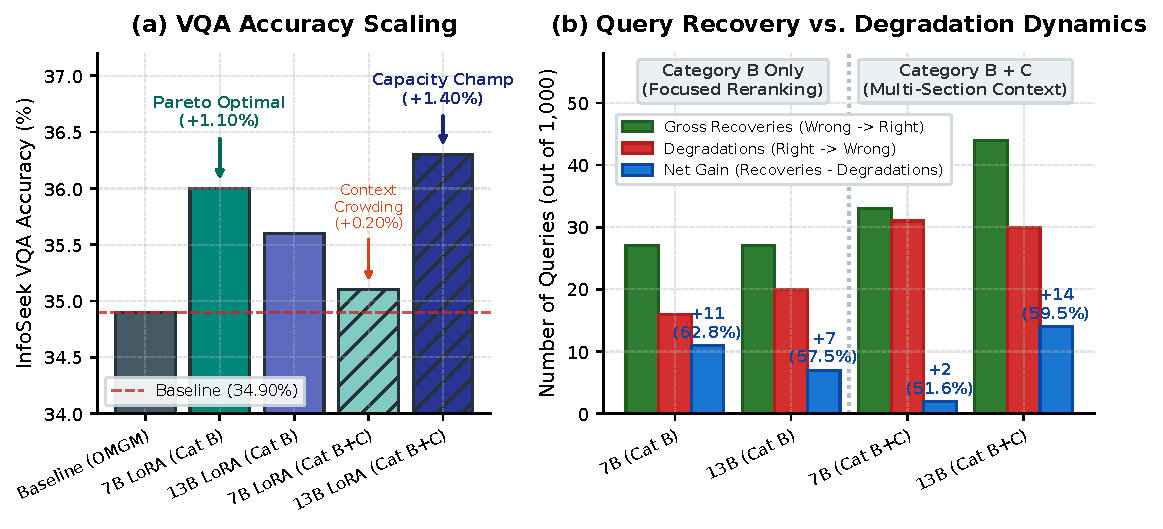
\includegraphics[width=\linewidth]{figs/fig3_scaling_matrix_double_dissociation}
\caption{The \texorpdfstring{$2 \times 2$}{2x2} capacity and task double dissociation across 1,000 test queries. Lightweight 7B models establish the Pareto frontier for pairwise verification (Cat B), while 13B models are structurally required to overcome distractor dilution during context expansion (Cat B+C).}
\label{fig:scaling_matrix}
\end{figure}

\subsection{The \texorpdfstring{$2 \times 2$}{2x2} Capacity \& Verification Double Dissociation}
Our benchmark across model scales (7B vs. 13B) and recovery formulations (Category~B vs. Category~B+C) reveals a striking \textbf{double dissociation} (Fig.~\ref{fig:scaling_matrix}):
(1)~\textbf{7B Wins on Category B (Pairwise Verification):} On focused visual adjudication between Candidate 1 and Candidate 2, fine-tuned 7B is remarkably agile, incurring only 16 degradations across 1,000 queries (62.8\% win-rate). In contrast, 13B's heavier semantic priors induce slight overconfidence (20 degradations). Consequently, \textbf{7B is Pareto-optimal for Category B}: achieving higher net accuracy (+1.10\% vs. +0.70\%), 44\% lower latency (3.24s vs. 4.67s), and 50\% lower VRAM consumption.
(2)~\textbf{13B Dominates on Category B+C (Context Expansion):} Concatenating Top-1 and Top-2 sections doubles prompt context to $\sim$3,200 characters. With 32 attention heads, 7B suffers from distractor dilution and ``lost in the middle'' degradation~\cite{liu2024lost}: in 14 queries, it hallucinated structural table headers (-6 net Cat C loss). In contrast, 13B's 40 attention heads isolate the relevant fact, yielding \textbf{18 Category C recoveries} against 10 degradations (+8 net gain), establishing Champion 13B at \textbf{36.30\% accuracy} (+14 net queries, 44 gross recoveries, capacity scaling advantage $\Delta\Delta = +16$ queries).

\subsection{Qualitative Analysis and Rescued Case Studies}
Adaptive Agentic Retrieval rescues queries failed by rigid baselines:
(1)~\textit{Geographical ($\mathtt{00000477}$):} For lake outflow, OMGM predicted Lake Z{\"u}rich ($\Delta = 0.009$); visual verification switched to \textit{Lake Lucerne}, yielding ``\textbf{Reuss}'' (Ground Truth: \textit{Reuss River}) $\to$ \textbf{[Recovered]}.
(2)~\textit{Waterway ($\mathtt{00013636}$):} For city water body, OMGM output ``Caspian Sea''; verifier switched to \textit{Kazan}, recovering ``\textbf{Volga}'' $\to$ \textbf{[Recovered]}.
(3)~\textit{Predecessors ($\mathtt{00015575}$):} For prior structure, OMGM predicted no information; verifier chose \textit{St. Peter's Basilica}, extracting ``\textbf{Old St. Peter's Basilica}'' $\to$ \textbf{[Recovered]}.
(4)~\textit{Attribution ($\mathtt{00044711}$):} For bridge designer, OMGM selected Myslbek; verifier identified \textit{Franz Joseph Bridge}, recovering ``\textbf{Rowland Mason Ordish}'' $\to$ \textbf{[Recovered]}.
(5)~\textit{Morphology (Cat C, $\mathtt{00000289}$):} For bird wingspan, OMGM hallucinated ``132''; context expansion to Section 2 morphology tables yielded ``\textbf{1.32 meters}'' (Ground Truth: 1.34, within $\pm 10\%$) $\to$ \textbf{[Recovered]}.
(6)~\textit{Nomenclature (Cat C, $\mathtt{00071549}$):} For mountain naming, OMGM predicted ``Denali''; Section 2 naming text produced ``\textbf{William McKinley}'' $\to$ \textbf{[Recovered]}.


\section{Discussion, Generalization, and Limitations}

\textbf{Data Disjointness \& Generalization:} Our audit between 6,000 fine-tuning pairs ($\mathcal{D}_{sym}$, OVEN) and 1,000 InfoSeek test queries establishes: (1) \textbf{100\% strict image disjointness} (0/983 test images seen during training); (2) \textbf{88.0\% entity disjointness} (528/600 unique test entities absent as training targets); and (3) \textbf{Generalization transfer}: \textbf{85.19\%} (23/27) of 7B and \textbf{90.91\%} (40/44) of 13B rescued queries involve completely unseen entities, proving symmetric LoRA functions as an open-world visual adjudicator rather than a memorization cache.

\textbf{Efficiency \& Deployment:}
(1) Fast-Path gating ($\tau = 0.025$) routes 49.2\% of queries with zero extra compute.
(2) The controller averages only \textbf{1.51 generator calls per query}.
(3) Dual Tesla T4 latency is 1.65s (7B) and 3.14s (Champion 13B).
(4) Under 4-bit NF4 double quantization, peak VRAM is $\sim$\textbf{4.1\,GB per GPU}, running on consumer hardware without enterprise clusters.

\textbf{Limitations \& Future Work:}
(1) \textit{Category A Retrieval Ceiling (15.30\%):} In 153 queries, ground-truth entities are absent from Step~1 coarse retrieval, bounding reranking recovery; future work will explore iterative multi-query search.
(2) \textit{Ultra-Large Scaling (70B+):} Extending agentic routing to 70B+ models may support multi-document reasoning over noisy passages.


\section{Conclusion}
In this paper, we addressed the rigid feed-forward failure mode in Knowledge-Based Visual Question Answering. Auditing 1,000 InfoSeek queries over 100,000 Wikipedia articles, we revealed that 40.8\% of errors stem from premature pruning of valid candidates, accompanied by a sharp $3.3\times$ score margin collapse ($\Delta = 0.0512 \to 0.0155$). We presented Adaptive Agentic Retrieval, isolating ambiguous queries via zero-cost gating ($\tau = 0.025$). Uncovering severe zero-shot VLM positional bias (17.5\%), we demonstrated that symmetric PEFT ($r=16$) eliminates positional bias to 1.33\% and raises adjudication accuracy to 90.33\%. Furthermore, our scaling analysis revealed a $2 \times 2$ double dissociation: 7B is Pareto-optimal for pairwise adjudication (+1.10\% net, 62.8\% win-rate), whereas 13B is necessary to resist distractor dilution during multi-section evidence expansion (+1.40\% net, 44 recoveries). Our champion model achieves 36.30\% VQA accuracy on InfoSeek under strict zero leakage, establishing a new state of the art in adaptive multimodal retrieval.

\begin{thebibliography}{22}
\footnotesize
\setlength{\itemsep}{1.2pt plus 0.5pt minus 0.5pt}

\bibitem{okvqa}
K.~Marino \textit{et~al.}, ``OK-VQA: A visual question answering benchmark requiring external knowledge,'' in \textit{Proc. IEEE/CVF Conf. Comput. Vis. Pattern Recognit. (CVPR)}, 2019, pp. 3195--3204.

\bibitem{infoseek}
Z.~Yang \textit{et~al.}, ``InfoSeek: A dataset for information-seeking questions with large-scale knowledge,'' in \textit{Proc. Conf. Empirical Methods Natural Lang. Process. (EMNLP)}, 2023, pp. 8948--8965.

\bibitem{oven}
H.~Hu \textit{et~al.}, ``Open-domain visual entity recognition: Towards recognizing millions of Wikipedia entities,'' in \textit{Proc. IEEE/CVF Conf. Comput. Vis. Pattern Recognit. (CVPR)}, 2023, pp. 12046--12055.

\bibitem{lewis2020rag}
P.~Lewis \textit{et~al.}, ``Retrieval-augmented generation for knowledge-intensive NLP tasks,'' in \textit{Proc. Adv. Neural Inf. Process. Syst. (NeurIPS)}, vol.~33, 2020, pp. 9459--9474.

\bibitem{omgm2025}
C.~Lin \textit{et~al.}, ``OMGM: Orchestrate multiple granularities and modalities for efficient multimodal retrieval,'' in \textit{Proc. 63rd Annu. Meeting Assoc. Comput. Linguistics (ACL)}, 2025, pp. 1--12.

\bibitem{clip}
A.~Radford \textit{et~al.}, ``Learning transferable visual models from natural language supervision,'' in \textit{Proc. 38th Int. Conf. Mach. Learn. (ICML)}, 2021, pp. 8748--8763.

\bibitem{blip2}
J.~Li \textit{et~al.}, ``BLIP-2: Bootstrapping language-image pre-training with frozen large language models and bimodal encoders,'' in \textit{Proc. 40th Int. Conf. Mach. Learn. (ICML)}, 2023, pp. 19730--19742.

\bibitem{llava15}
H.~Liu \textit{et~al.}, ``Improved baselines with visual instruction tuning,'' in \textit{Proc. IEEE/CVF Conf. Comput. Vis. Pattern Recognit. (CVPR)}, 2024, pp. 26296--26306.

\bibitem{vqa_v2}
Y.~Goyal \textit{et~al.}, ``Making the V in VQA matter: Elevating the role of image understanding in Visual Question Answering,'' in \textit{Proc. IEEE Conf. Comput. Vis. Pattern Recognit. (CVPR)}, 2017, pp. 6904--6913.

\bibitem{aokvqa}
D.~Schwenk \textit{et~al.}, ``A-OKVQA: A benchmark for visual question answering using world knowledge,'' in \textit{Proc. Eur. Conf. Comput. Vis. (ECCV)}, 2022, pp. 146--162.

\bibitem{bge_reranker}
J.~Chen \textit{et~al.}, ``BGE M3-embedding: Multi-lingual, multi-functionality, multi-granularity text embeddings through self-knowledge distillation,'' \textit{arXiv:2402.03216}, 2024.

\bibitem{selfrag}
A.~Asai \textit{et~al.}, ``Self-RAG: Learning to retrieve, generate, and critique through self-reflection,'' in \textit{Proc. 12th Int. Conf. Learn. Represent. (ICLR)}, 2024.

\bibitem{crag}
S.-Q.~Yan \textit{et~al.}, ``Corrective retrieval augmented generation,'' \textit{arXiv:2401.15884}, 2024.

\bibitem{adaptiverag}
S.~Jeong \textit{et~al.}, ``Adaptive-RAG: Determining when and how to retrieve for knowledge-intensive language models,'' in \textit{Proc. Conf. North Amer. Chapter Assoc. Comput. Linguistics (NAACL)}, 2024, pp. 798--812.

\bibitem{jiang2023flare}
Z.~Jiang \textit{et~al.}, ``Active retrieval augmented generation,'' in \textit{Proc. Conf. Empirical Methods Natural Lang. Process. (EMNLP)}, 2023, pp. 7969--7992.

\bibitem{react}
S.~Yao \textit{et~al.}, ``ReAct: Synergizing reasoning and acting in language models,'' in \textit{Proc. 11th Int. Conf. Learn. Represent. (ICLR)}, 2023.

\bibitem{toolformer}
T.~Schick \textit{et~al.}, ``Toolformer: Language models can teach themselves to use tools,'' in \textit{Proc. Adv. Neural Inf. Process. Syst. (NeurIPS)}, vol.~36, 2023, pp. 68539--68551.

\bibitem{primacy_bias}
P.~Wang \textit{et~al.}, ``Large language models are not fair evaluators,'' in \textit{Proc. 62nd Annu. Meeting Assoc. Comput. Linguistics (ACL)}, 2024, pp. 9440--9450.

\bibitem{peiss_order_bias}
P.~Pezeshkpour and E.~Hruschka, ``Large language models sensitivity to the order of options in multiple-choice questions,'' in \textit{Findings of Assoc. Comput. Linguistics: NAACL 2024}, 2024, pp. 2019--2034.

\bibitem{lora}
E.~J.~Hu \textit{et~al.}, ``LoRA: Low-rank adaptation of large language models,'' in \textit{Proc. 10th Int. Conf. Learn. Represent. (ICLR)}, 2022.

\bibitem{qlora}
T.~Dettmers \textit{et~al.}, ``QLoRA: Efficient finetuning of quantized LLMs,'' in \textit{Proc. Adv. Neural Inf. Process. Syst. (NeurIPS)}, vol.~36, 2023, pp. 10088--10115.

\bibitem{liu2024lost}
N.~F.~Liu \textit{et~al.}, ``Lost in the middle: How language models use long contexts,'' \textit{Trans. Assoc. Comput. Linguistics}, vol.~12, pp. 157--173, 2024.

\end{thebibliography}

\end{document}
